\section{Use Case}
\label{sec:UseCase}

For the purposes of this milestone, we explore the problem of
characterizing fragments in an explosion simulation.  Simulation is a vital
part in understanding shock physics.  Although experimentation will always
be a necessary tool for scientific inquiry and corroboration, the amount of
data we can retrieve with experimentation is limited.  Experiments in shock
physics usually involve high energy, high velocities, and high variability,
all of which hinder detailed, accurate, and repeatable observations during
the experiment.  When measurements cannot be taken during the experiment,
they must be taken after the experiment by observing the remaining
material.  Much can be learned in the manner, but the transient states
during the experiment are lost.

Another limiting factor of experimentation is its high cost and slow
turnaround.  To create shock physics experiments, physical devices must be
fabricated.  These devices are then usually destroyed during the
experiment.  Safety and political issues also often plague shock physics
experiments.  In some cases, experimentation is simply not feasible.  Thus,
simulation plays a major role in shock physics analysis.

In this milestone, we use an example simulation of an exploding pipe shown
in Figure~\ref{fig:ExplodingPipe}.  This similation problem is provided to
our group by Jason Wilke.  In addition to well representing the kinds of
simulation and analysis done at Sandia National Laboratories, this
simulation provides interesting results and many different levels of
refinement, which allows us to scale the problem from less than 100 cores
to well over 10,000 cores.

\begin{figure}[htb]
  \centering
  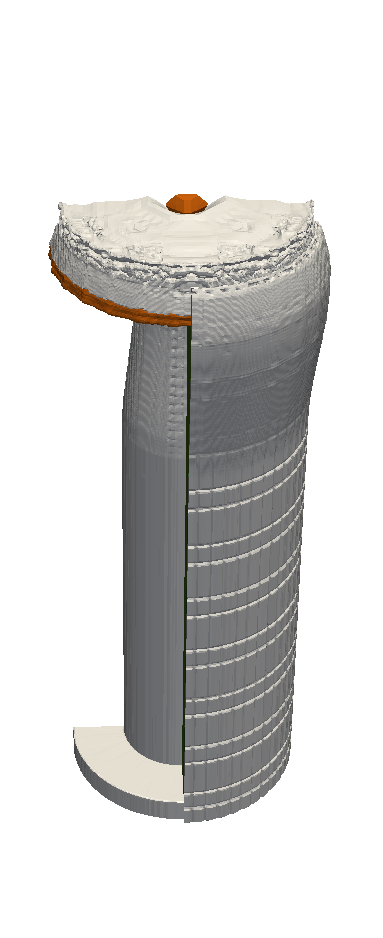
\includegraphics[height=3in]{figures/pipe_25}
  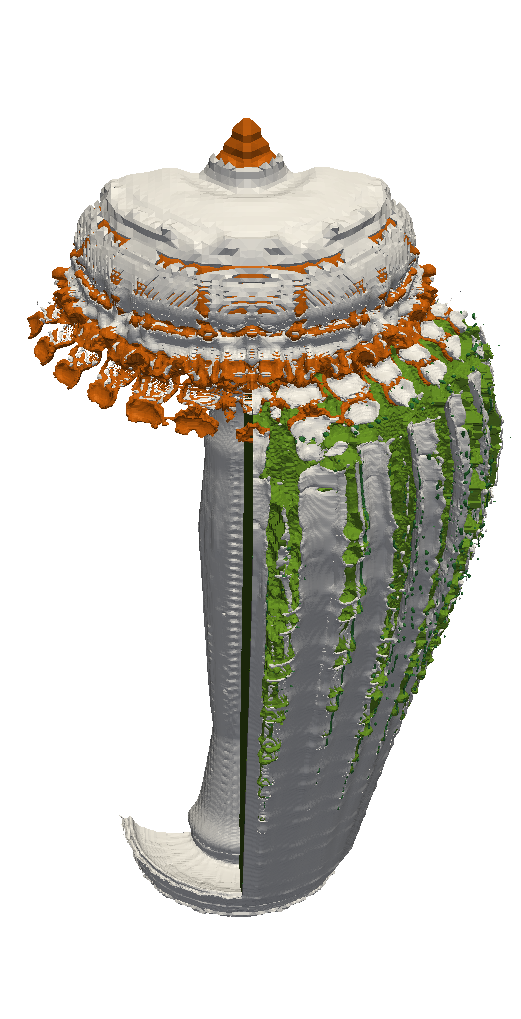
\includegraphics[height=3in]{figures/pipe_75}
  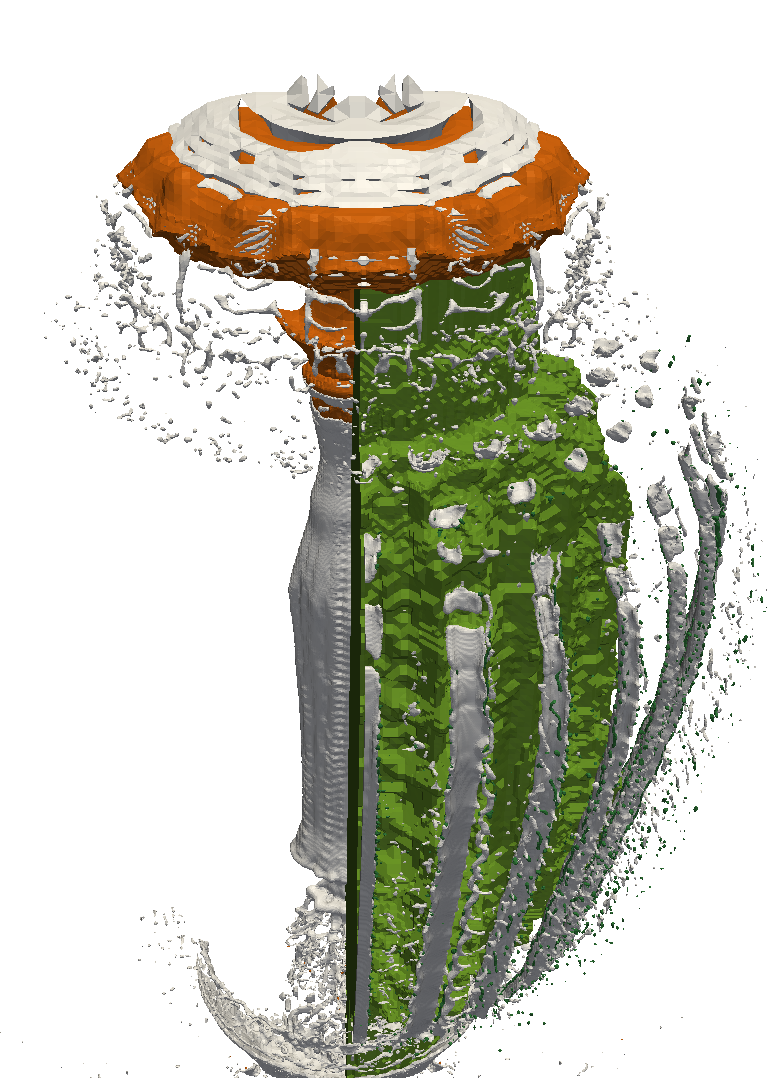
\includegraphics[height=3in]{figures/pipe_125}
  \caption[Simulation of an exploding pipe.]{Simulation of an exploding
    pipe, which presents many prototypical fragment analysis challenges.}
  \label{fig:ExplodingPipe}
\end{figure}

One of the most important features in shock physics analysis is material
fragments.  The physical properties of the fragments, including mass,
volume, and shape, as well as their trajectories, can all be important.  In
particular, shape can be an important characteristic.  Consider the example
fragments given in Figure~\ref{fig:Fragments}.  The top fragment is long
and sharp, making it more likely to penetrate objects.  In comparison, the
bottom left fragment is rounded and could have less damage potential.
However, the U-shaped fragment in the bottom right may be harmful depending
on the scenario, but could be difficult to distinguish from the round
fragment in many shape metrics.

\begin{figure}[htb]
  \centering
  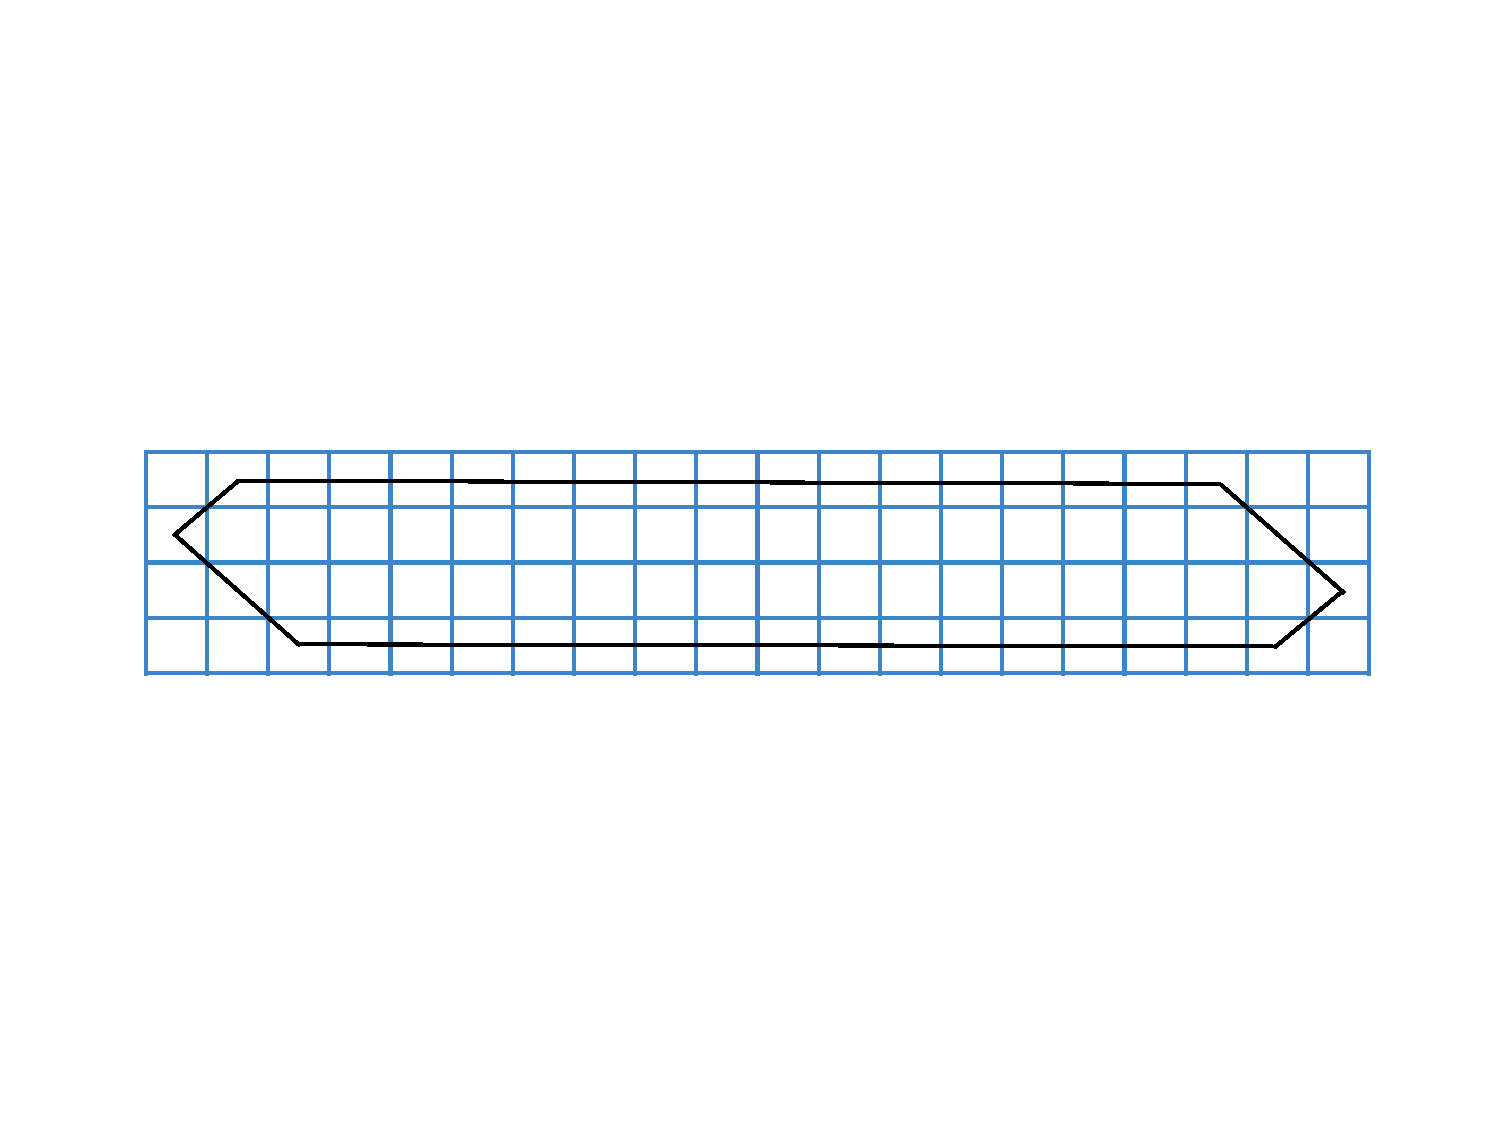
\includegraphics[trim=0cm 5.5cm 0cm 5.5cm,clip=true,width=.9\linewidth]{figures/Fragment-Sharp}
  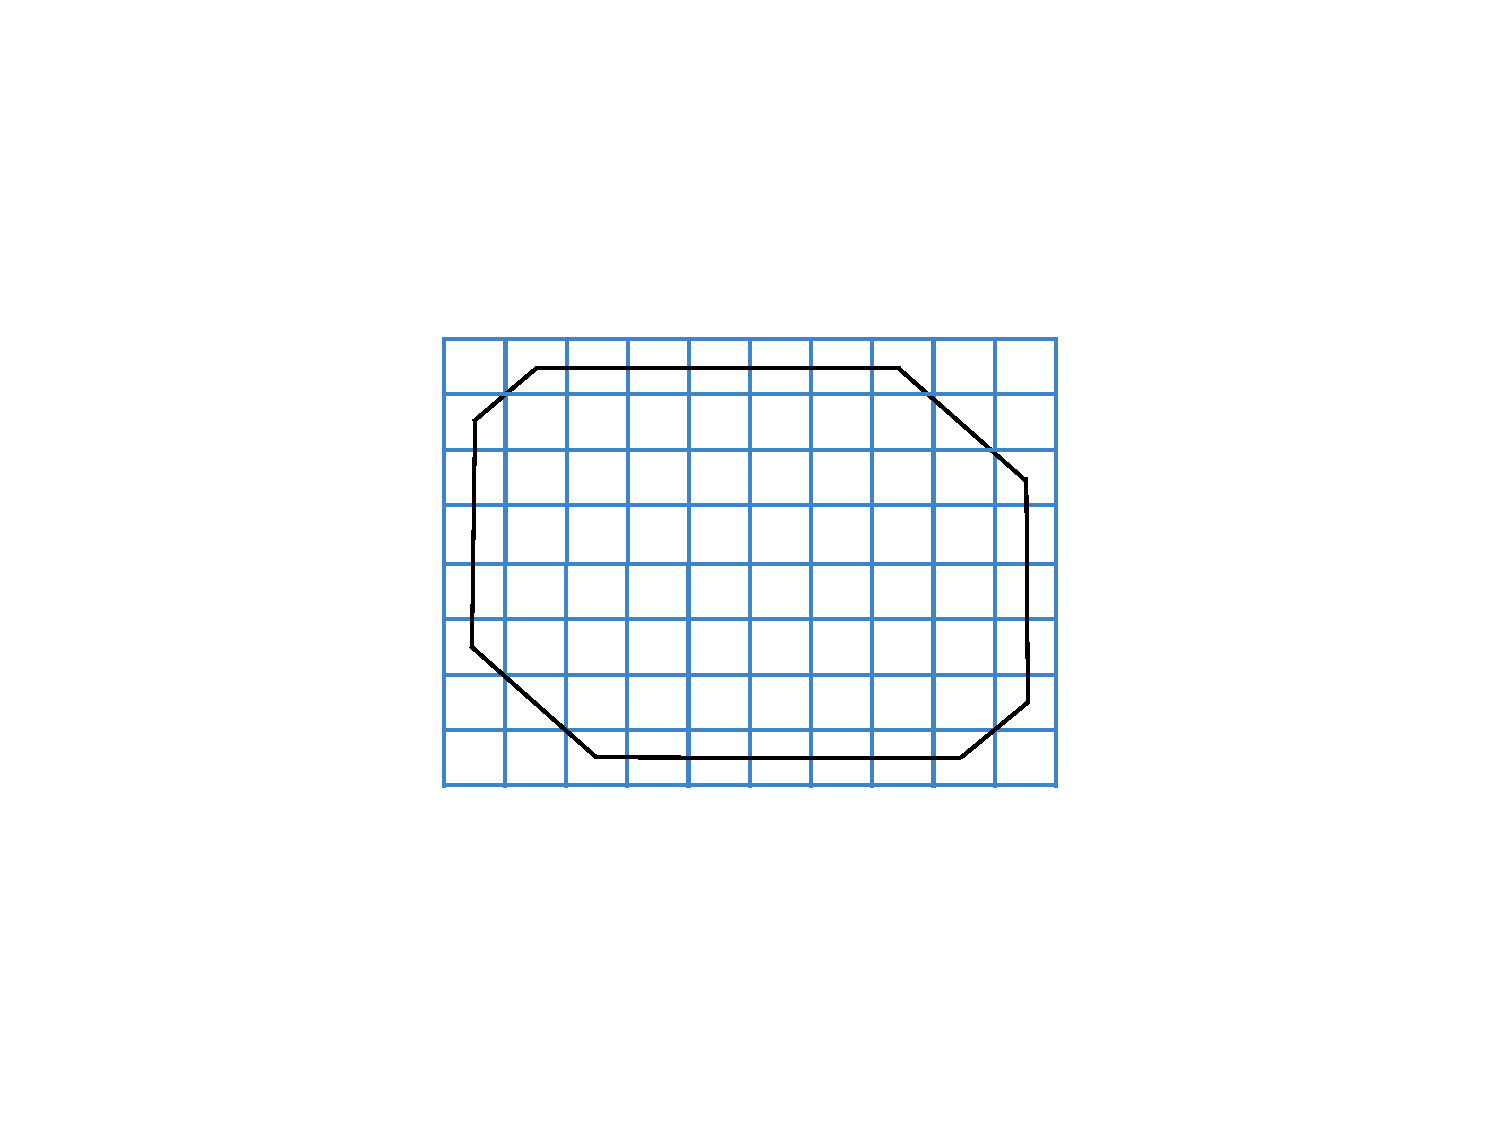
\includegraphics[trim=5.5cm 5.5cm 5.5cm 5.5cm,clip=true,width=.4\linewidth]{figures/Fragment-Rounded}
  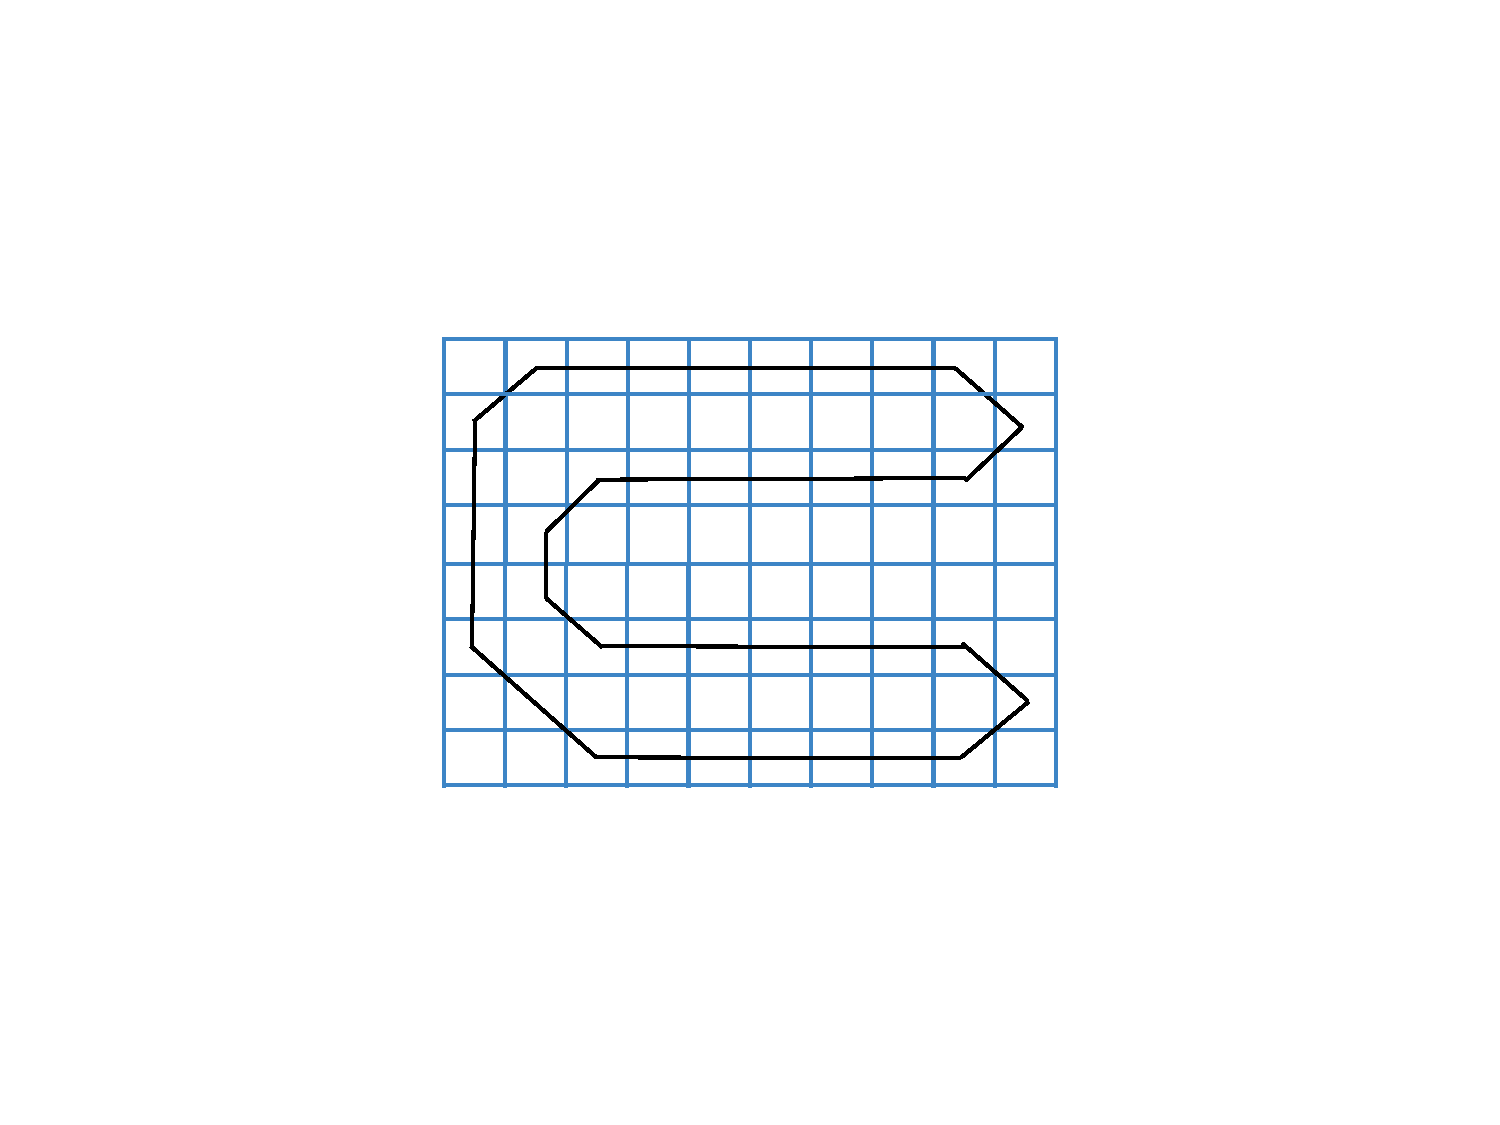
\includegraphics[trim=5.5cm 5.5cm 5.5cm 5.5cm,clip=true,width=.4\linewidth]{figures/Fragment-Ushaped}
  \caption[Examples of potential fragments.]{Examples of potential
    fragments that we would like to characterize.}
  \label{fig:Fragments}
\end{figure}

The simulation code we use is CTH\lcite{CTH,CTHAMR}.  It is an Eulerian
shock physics code that uses an adaptive mesh refinement (AMR) data model.
These adaptive finite volumes can take up different amounts of space
depending on where they are in the model and how closely the simulation is
refining the space.

In order to correctly find fragments, we must first determine what is and
is not a fragment.  The simulation operates on a finite volume and
comprises a set of simulated materials, which each take up a certain
fraction of finite cells within that volume.  We treat any connected region
of cells with material volume fraction above a given threshold as a
fragment of that material.  Generally speaking, when a simulation begins,
each material comprises usually one connected region, which we refer to as
the main mass.  As the simulation progresses, this region breaks apart and
gaps occur between pieces of material, filled either by another material or
by the surrounding air.  Once there is a gap as wide as at least one cell,
we determine that a fragment as formed.  The challenge when finding these
fragments on a large scale parallel system is that regions that make up the
fragments straddle process boundaries, requiring communication between the
processes to determine the full shape of a fragment.

Because the number of fragments a shock physics simulation can generate are
so numerous, it is seldom realistic for a person to examine every one.  It
is therefore more beneficial to first perform computational analytics that
provide useful summary statistics and identify particularly interesting
fragments.  This analysis has the added benefit of reducing the amount of
memory required to represent it.  Therefore, fragment analysis is a good
candidate for \insitu processing.

A full fragment analysis requires multiple steps.
\begin{enumerate}
\item Identify the boundaries of fragments.  This transition over the
  volume fraction threshold allows us to separate what is and is not a
  fragment.
\item Find the fragment connected components.  A connected components
  analysis brings together all finite elements that belong to a single
  fragment.
\item Characterize properties of fragments.  Given the collected elements
  for each fragment, find the features such as shape volume, and movement
  that are of interest.
\item Extract useful information.  This could involve, for example,
  computing histograms of features or extracting a small subset of
  fragments deemed important.
\end{enumerate}

\emph{For the purpose of simplifying the problem and making it tractable
  for analysis, we abbreviate the problem to include only the
  identification of fragment boundaries} for the results of this milestone.
The creation of fragment boundaries is a nontrivial problem in that we must
make sure the surface is ``watertight'' in that the representative mesh
surface is conforming and closed.  Making a surface from an AMR mesh
watertight is challenging because the AMR mesh itself is nonconforming at
boundaries between adjacent regions at different levels of refinement.

\begin{figure}[htb]
  \centering
  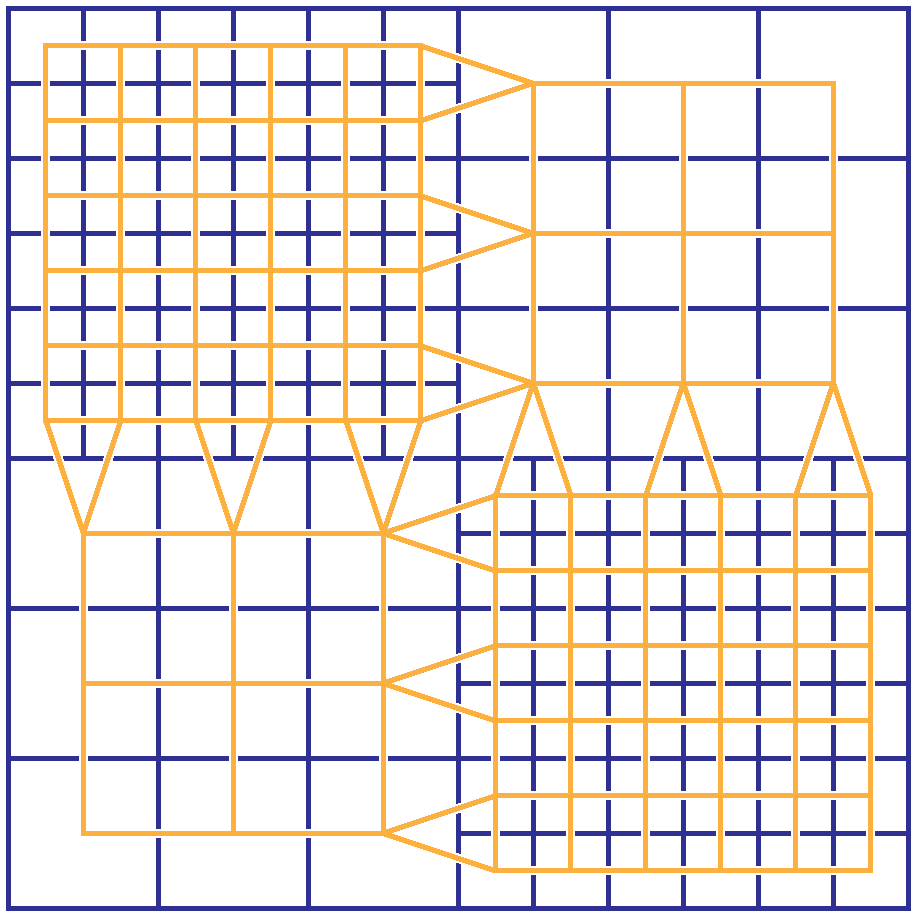
\includegraphics[width=5in]{figures/AMRDual}
  \caption[A simple 2D AMR example.]{A simple 2D AMR example with 2
    different refinement levels (blue lines) and the conforming dual grid
    we build with it (yellow lines).}
  \label{fig:AMRDual}
\end{figure}

To generate this watertight fragment surface, we first build a dual mesh of
the original AMR mesh.  The dual mesh contains a vertex at the center of
each cell in the original mesh and an edge through each face of of the
original mesh as demonstrated in Figure~\ref{fig:AMRDual}.  The advantage
of creating a dual mesh is that it is straightforward to build conforming
cells across the boundaries of AMR regions with different levels of
refinement.

The disadvantage of building these dual meshes in a distributed parallel
job is that neighborhood information must be shared between regions that
might be located on different processes.  Resolving this neighborhood
information requires a significant amount of communication.  (Such
communication would be necessary for any creation of a watertight mesh.)
This communication can limit the scalability of the algorithm.

Efficient communication of boundary elements first requires that each
process knows the location of the neighbors for each region it holds.  If
data is loaded with no knowledge of its decomposition, which is typical in
the post-processing of data, then this neighborhood information can be
retrieved only through global communication.  Our initial
\keyterm{baseline} algorithm starts with this global communication, which
we find to severely limit the scalability of the algorithm.

However, when running the surface creation algorithm as an embedded \insitu
component of CTH, this global communication of finding neighbors is
wasteful because CTH already has this information.  To take advantage of
this neighborhood information, we make a small change to CTH to pass this
data decomposition information through its I/O layer to Catalyst.  With
this data, our \keyterm{refined} algorithm skips the global communication
leaving only the more scalable boundary-data passing.  Our analysis shows
that the refined algorithm is much more scalable than the baseline
algorithm\lcite{Fabian2012}.  Unfortunately, we cannot apply the refined
algorithm in the \intransit workflow because this workflow redistributes
the data and invalidates this neighborhood information from CTH.
